\appendix{Description of BER Test Setup}
\label{sec:appendxi_setup}
The major components from the block diagram shown in Figure \ref{fig:LabTestBlock} functions are summarized as follows:
\begin{itemize}
\item The \textbf{SOQPSK-TG Transmitter} is a PAQ enabled L-band transmitter shown in Figure \ref{fig:trans}.
\item The \textbf{Multipath Channel} emulator generates multipath interference for a given channel at RF shown in Figure \ref{fig:emu}.
\item The \textbf{Noise Source} generates calibrated additive white Gaussian noise for a given $\text{E}_\text{b}/\text{N}_\text{0}$ shown in Figure \ref{fig:noise}.
\item The \textbf{Power Splitter} split the power between the Spectrum Analyzer and the T/M Receiver \& Demodulator  shown in Figure \ref{fig:splitter}.
\item The \textbf{Spectrum Analyzer} showed the power spectrum of the multipath channel shown in Figure \ref{fig:specAn}.
\item The \textbf{T/M Receiver \& Demodulator} produced the no equalization bits at $10.3125$ Mbits/s and down-converted RF to $70$ MHz IF  shown in Figure \ref{fig:HostSystem}.
\item The \textbf{Preamble Scrubber} explained in \cite{hog2016} locates and removes the preamble and ASM in the $10.3125$ Mbits/s to produce a data bit stream at $10$ Mbits/s shown in Figure \ref{fig:scrubber}.
\item The \textbf{BERT} computes the BER for six bit streams shown in Figure \ref{fig:HostSystem}.
\end{itemize}
\clearpage
\begin{figure}
	\centering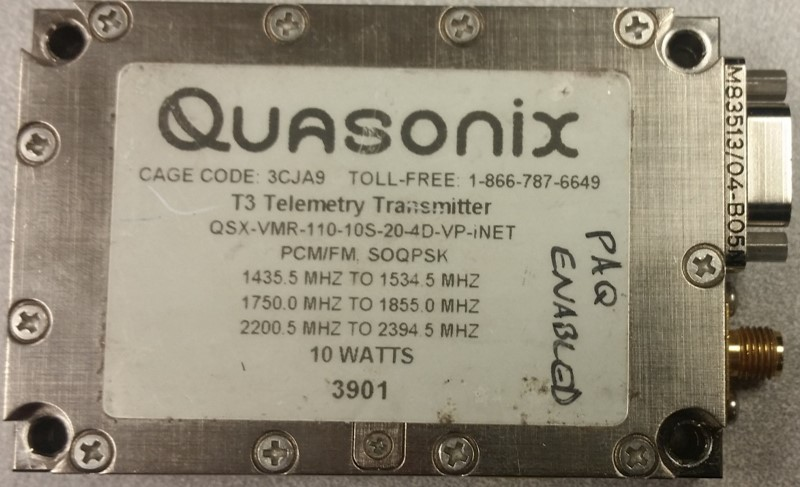
\includegraphics[scale=0.5]{figures/eq_GPUimplementation/trans.jpg}
	\caption{PAQ enabled L-band transmitter QSX VMR 110 00S 20 2D VP iNET S/N 3901.}
	\label{fig:trans}
\end{figure}
\begin{figure}
	\centering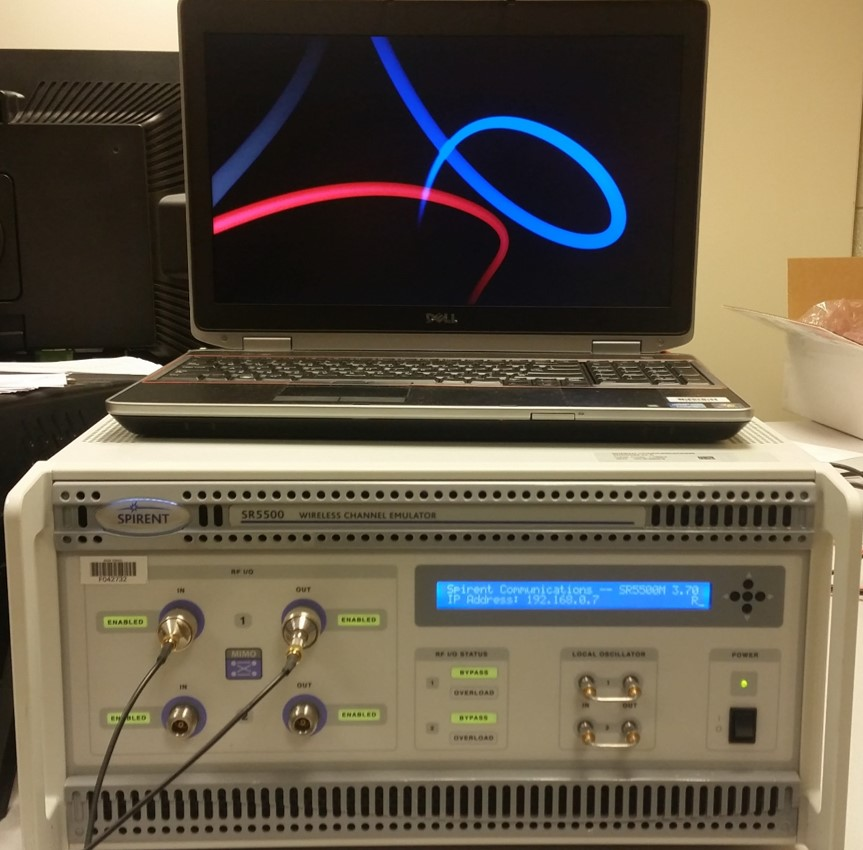
\includegraphics[scale=0.5]{figures/eq_GPUimplementation/emu.jpg}
	\caption{Channel emulator Spirint SR 5500 Wireless Channel Emulator.}
	\label{fig:emu}
\end{figure}
\begin{figure}
	\centering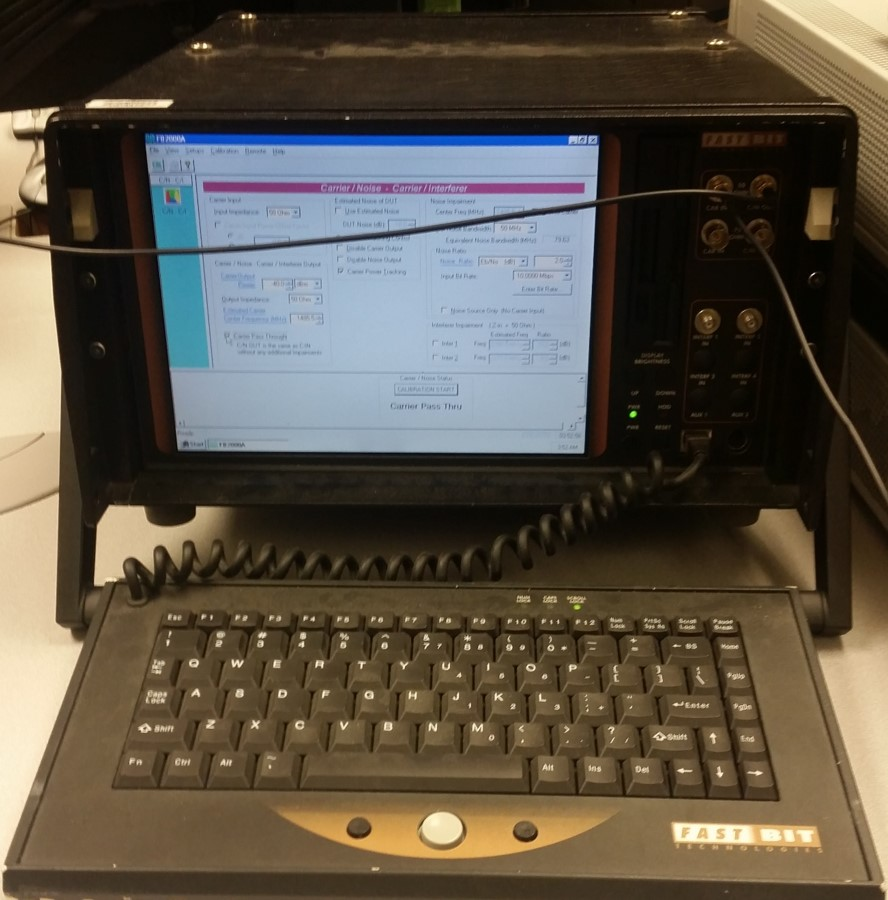
\includegraphics[scale=0.5]{figures/eq_GPUimplementation/noise.jpg}
	\caption{Noise source Fast Bit FB0008.}
	\label{fig:noise}
\end{figure}
\begin{figure}
	\centering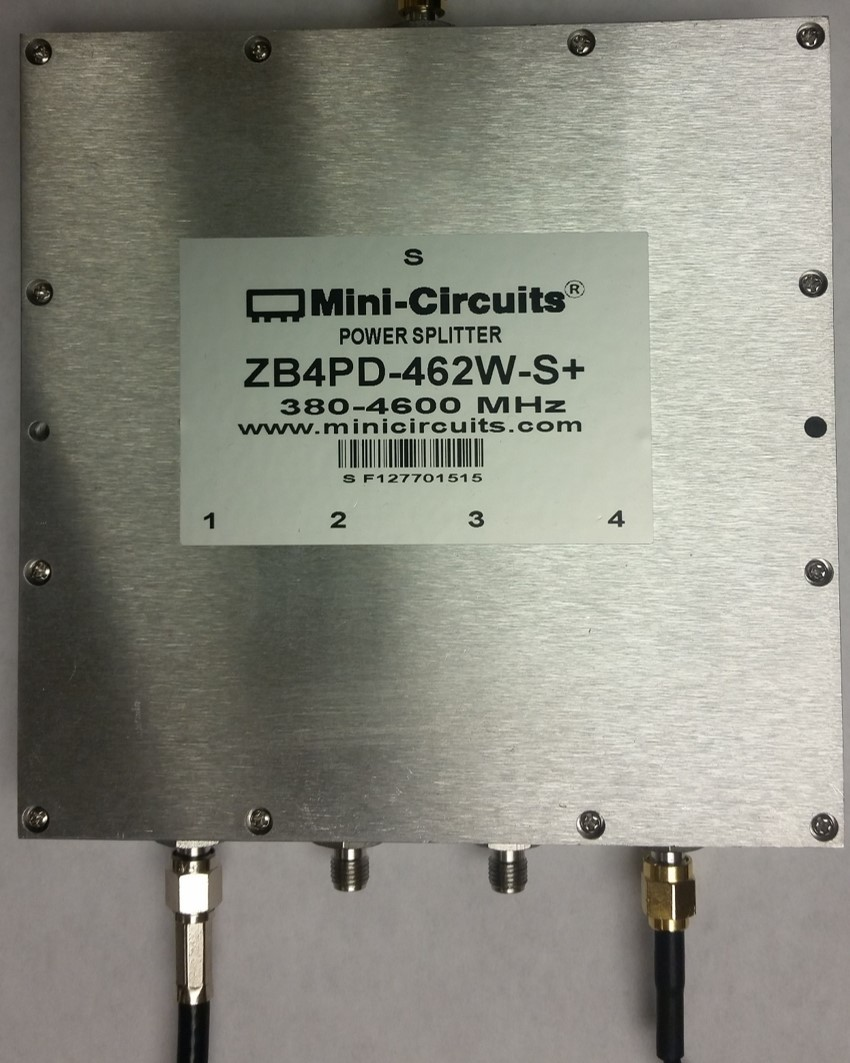
\includegraphics[scale=0.5]{figures/eq_GPUimplementation/splitter.jpg}
	\caption{Power splitter Mini-circuits ZB4PD-462W-S+.}
	\label{fig:splitter}
\end{figure}
\begin{figure}
	\centering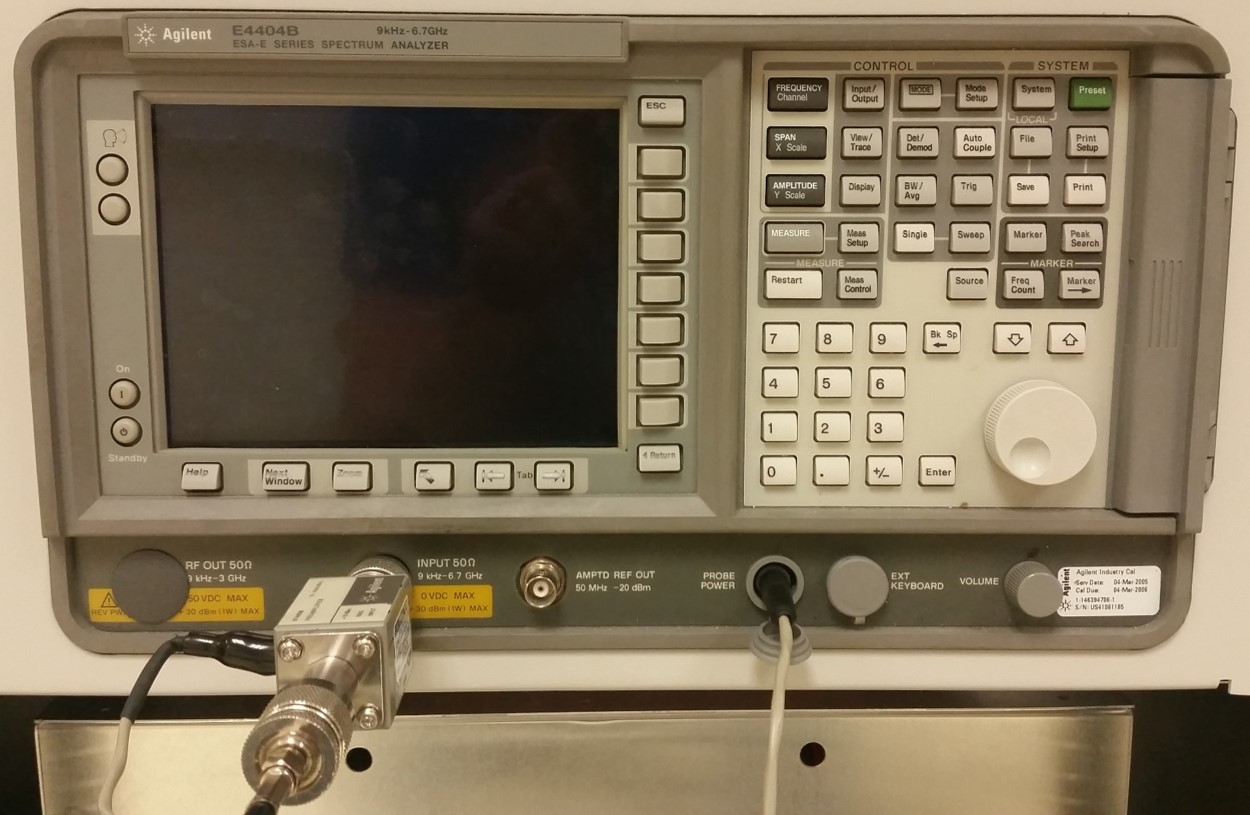
\includegraphics[scale=0.5]{figures/eq_GPUimplementation/specAn.jpg}
	\caption{Spectrum analyzer Agilent E4404B ESA-E Series Spectrum Analyzer.}
	\label{fig:specAn}
\end{figure}
\begin{figure}
	\centering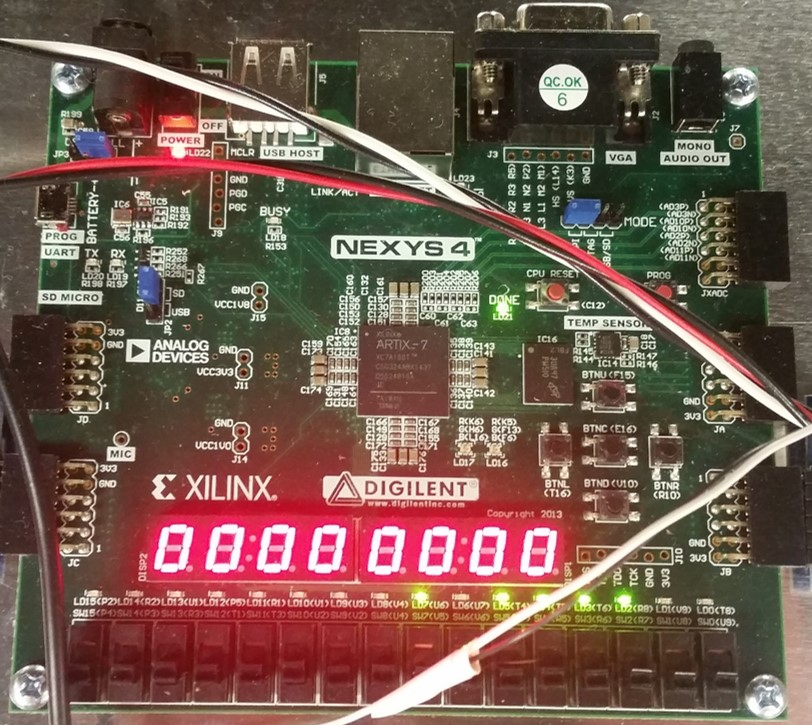
\includegraphics[scale=0.5]{figures/eq_GPUimplementation/scrubber.jpg}
	\caption{Preamble and ASM scrubber.}
	\label{fig:scrubber}
\end{figure}